% !TEX root = ../DP_Vik_Tomas_2013.tex
\chapter{Výsledky dotazníku pro vyhodnocení UI}
\label{chp:vysledky}
V této příloze jsou pouze čistě výsledky dotazníku, jejich vyhodnocení se nachází v kapitole \ref{sec:vyhodnoceni-dotazniku}. Ve schématech znamenají tučná čísla počet respondentů. Celkem jich bylo \textbf{22}.

\section{Základní dotazník}
Výsledky odpovědí na základní SUS dotazník.
Všechny odpovědi jsou hodnocené na stupnici 1-Vůbec nesouhlasím až 5-Plně souhlasím.

\begin{figure}[H]
\begin{center}
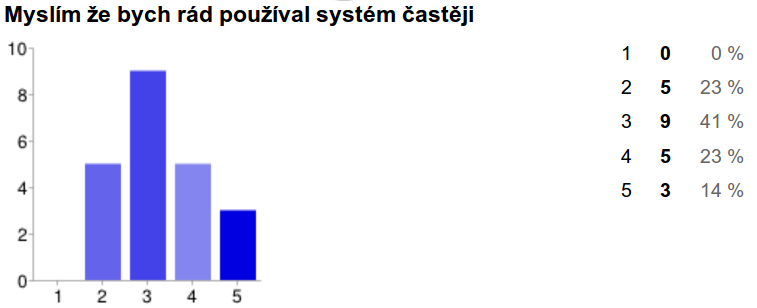
\includegraphics[width=80mm]{./pictures/dotaznik/sus-01.png}
%\caption{Graf s výsledky první otázky}
\label{fig:dot:sus-01}
\end{center}
\end{figure}

\begin{figure}[H]
\begin{center}
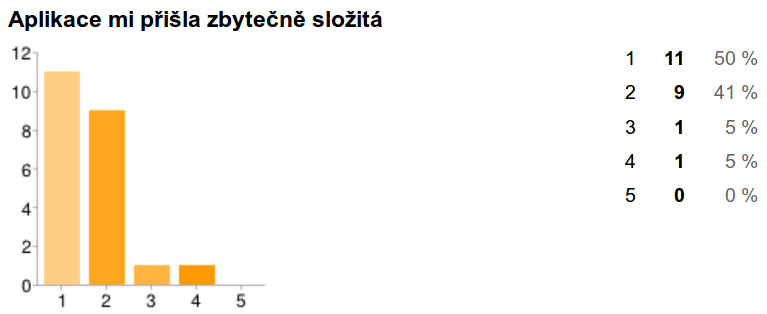
\includegraphics[width=80mm]{./pictures/dotaznik/sus-02.png}
%\caption{Graf s výsledky druhé otázky}
\label{fig:dot:sus-02}
\end{center}
\end{figure}

\begin{figure}[H]
\begin{center}
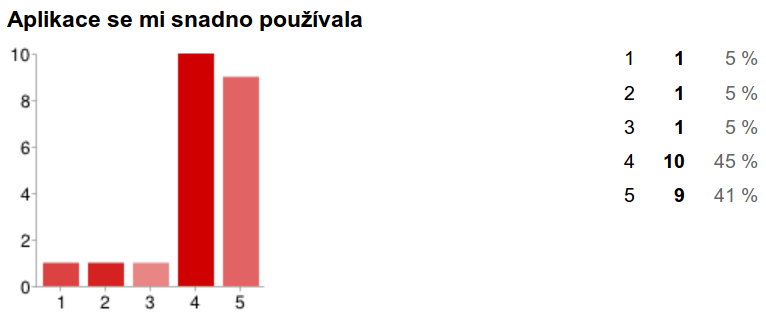
\includegraphics[width=80mm]{./pictures/dotaznik/sus-03.png}
%\caption{Graf s výsledky třetí otázky}
\label{fig:dot:sus-03}
\end{center}
\end{figure}

\begin{figure}[H]
\begin{center}
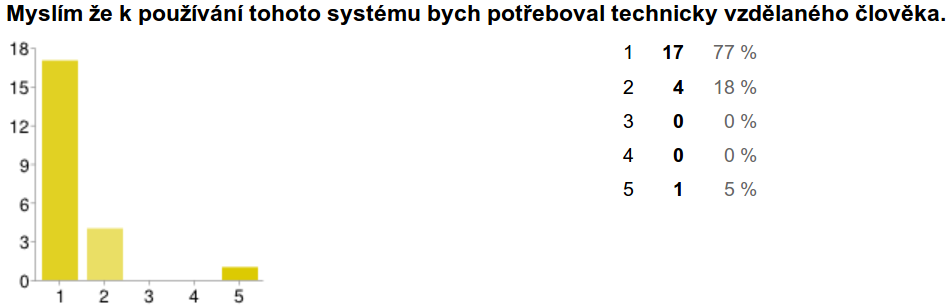
\includegraphics[width=80mm]{./pictures/dotaznik/sus-04.png}
%\caption{Graf s výsledky čtvrté otázky}
\label{fig:dot:sus-04}
\end{center}
\end{figure}

\begin{figure}[H]
\begin{center}
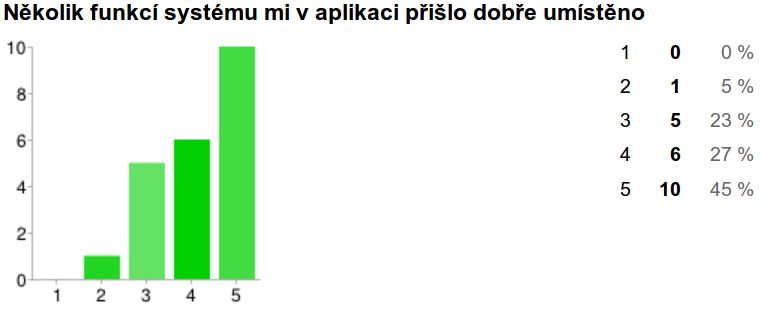
\includegraphics[width=80mm]{./pictures/dotaznik/sus-05.png}
%\caption{Graf s výsledky páté otázky}
\label{fig:dot:sus-05}
\end{center}
\end{figure}

\begin{figure}[H]
\begin{center}
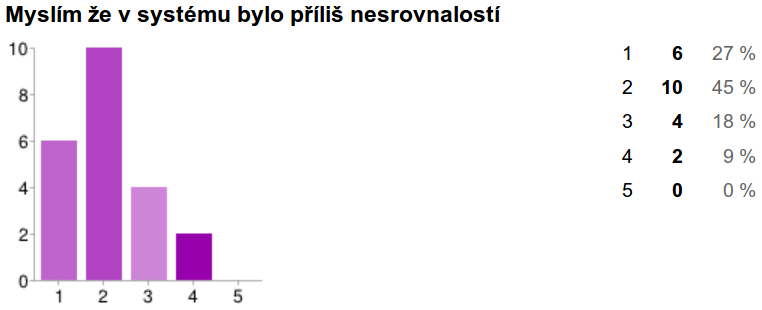
\includegraphics[width=80mm]{./pictures/dotaznik/sus-06.png}
%\caption{Graf s výsledky šesté otázky}
\label{fig:dot:sus-06}
\end{center}
\end{figure}

\begin{figure}[H]
\begin{center}
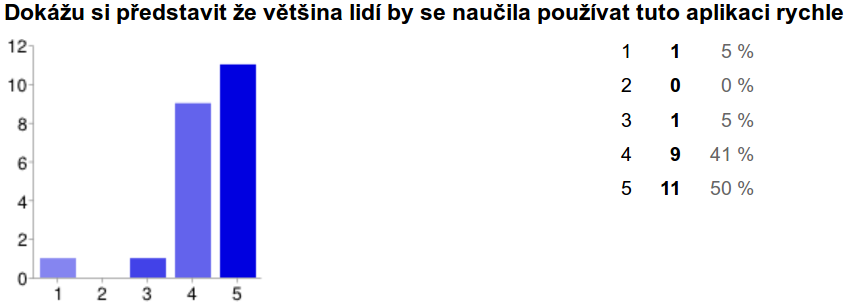
\includegraphics[width=80mm]{./pictures/dotaznik/sus-07.png}
%\caption{Graf s výsledky sedmé otázky}
\label{fig:dot:sus-07}
\end{center}
\end{figure}

\begin{figure}[H]
\begin{center}
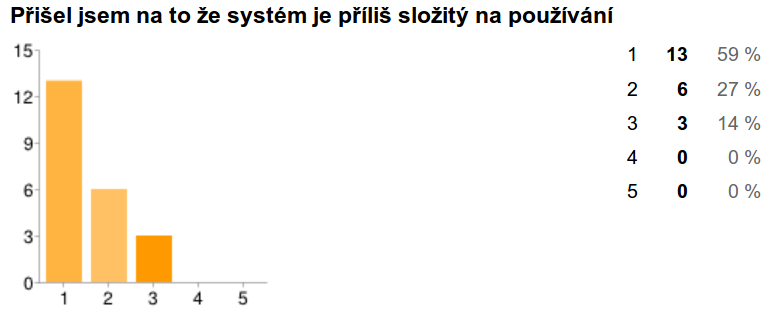
\includegraphics[width=80mm]{./pictures/dotaznik/sus-08.png}
%\caption{Graf s výsledky osmé otázky}
\label{fig:dot:sus-08}
\end{center}
\end{figure}

\begin{figure}[H]
\begin{center}
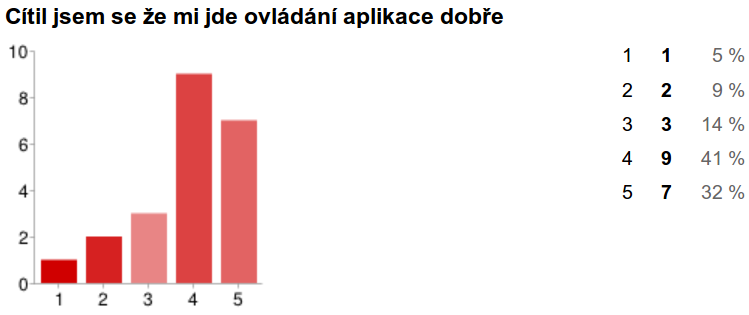
\includegraphics[width=80mm]{./pictures/dotaznik/sus-09.png}
%\caption{Graf s výsledky deváté otázky}
\label{fig:dot:sus-09}
\end{center}
\end{figure}

\begin{figure}[H]
\begin{center}
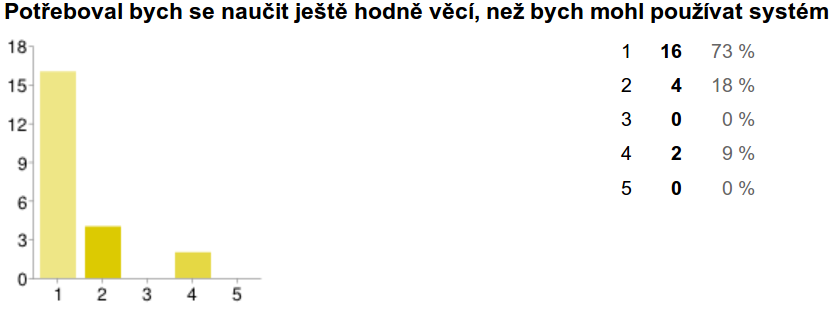
\includegraphics[width=80mm]{./pictures/dotaznik/sus-10.png}
%\caption{Graf s výsledky desáté otázky}
\label{fig:dot:sus-10}
\end{center}
\end{figure}

\section{Pokročilý dotazník}
U otázky \emph{Pochopil jsi na co aplikace slouží?} znamenají odpovědi 1=vůbec nebo s velkými problémy až 5=okamžitě bez problému. U otázky \emph{Bylo náročné přidat předmět přání?} znamenají odpověďi 1=nepřišel jsem na to jak až 5=byla to hračka.
Od výsledků poslední otázky se odvíjelo, na jaké další otázky bude uživatel odpovídat (např. pokud uživatel nepřidal ani jedno přání, nemá smysl se ho ptát na to zdali přesouval přání ve svém seznamu). Proto je tato část poslední, kde odpovídalo všech 22 respondentů.

\begin{figure}[H]
\begin{center}
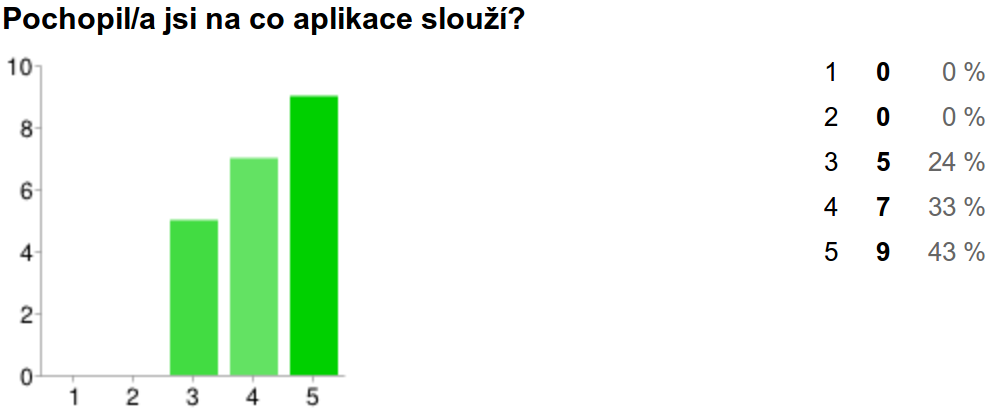
\includegraphics[width=80mm]{./pictures/dotaznik/pokrocily-01.png}
\label{fig:dot:pokrocily-01}
\end{center}
\end{figure}

\begin{figure}[H]
\begin{center}
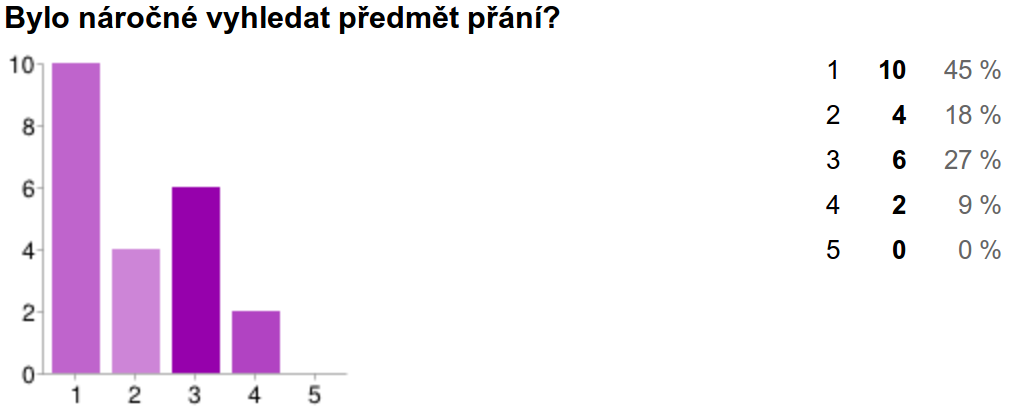
\includegraphics[width=80mm]{./pictures/dotaznik/pokrocily-02.png}
\label{fig:dot:pokrocily-02}
\end{center}
\end{figure}

\begin{figure}[H]
\begin{center}
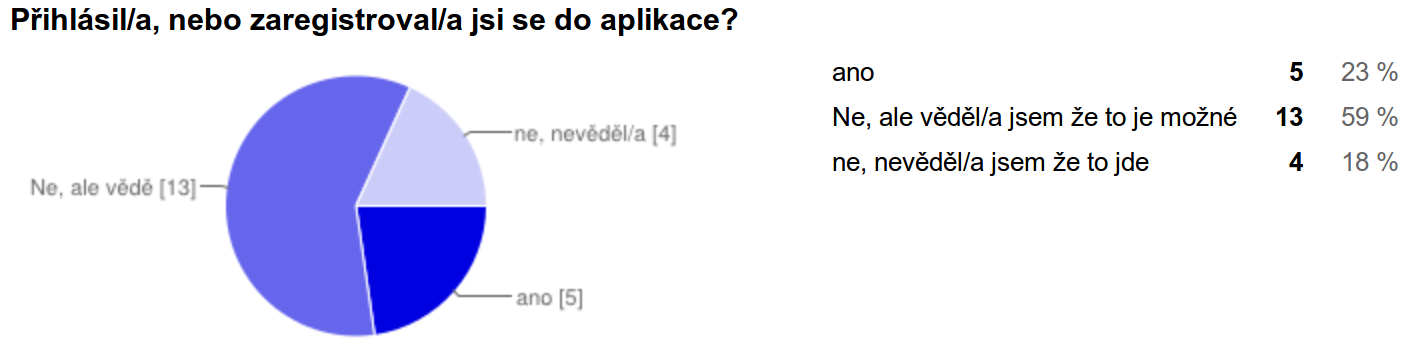
\includegraphics[width=120mm]{./pictures/dotaznik/pokrocily-03.png}
\label{fig:dot:pokrocily-03}
\end{center}
\end{figure}

\begin{figure}[H]
\begin{center}
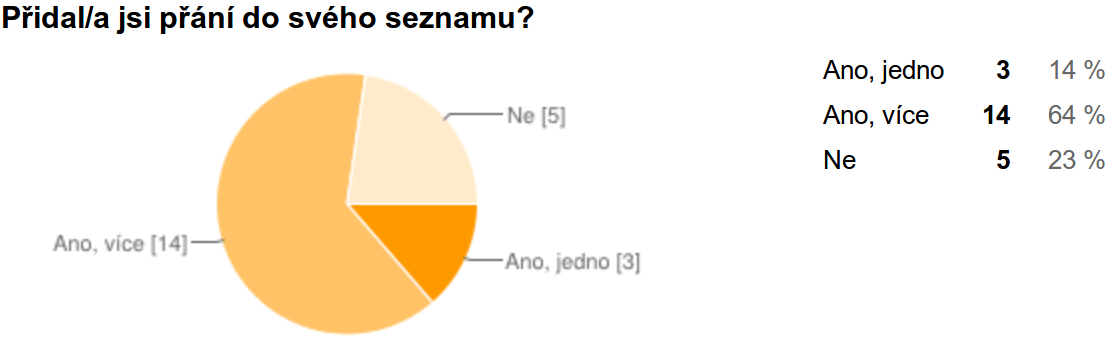
\includegraphics[width=100mm]{./pictures/dotaznik/pokrocily-04.png}
\label{fig:dot:pokrocily-04}
\end{center}
\end{figure}


\section{Práce s přáními}
Do této kategorie přispívali pouze respondenti, kteří v předchozí části dotazníku odpověděli, že do svého seznamu přidali více než jedno přání.
\begin{figure}[H]
\begin{center}
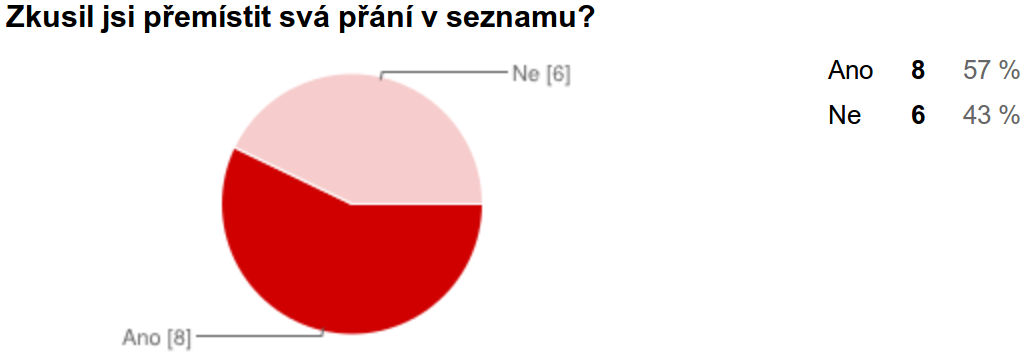
\includegraphics[width=110mm]{./pictures/dotaznik/vice-prani-01.png}
\label{fig:dot:vice-prani-01}
\end{center}
\end{figure}

\begin{figure}[H]
\begin{center}
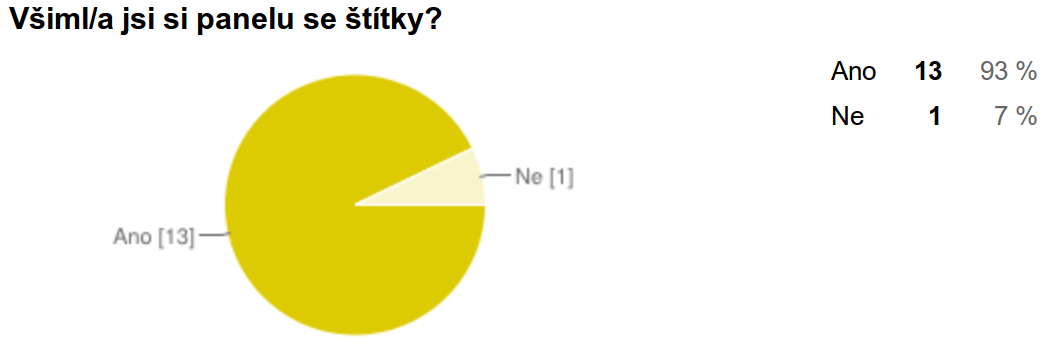
\includegraphics[width=110mm]{./pictures/dotaznik/vice-prani-02.png}
\label{fig:dot:vice-prani-02}
\end{center}
\end{figure}

\begin{figure}[H]
\begin{center}
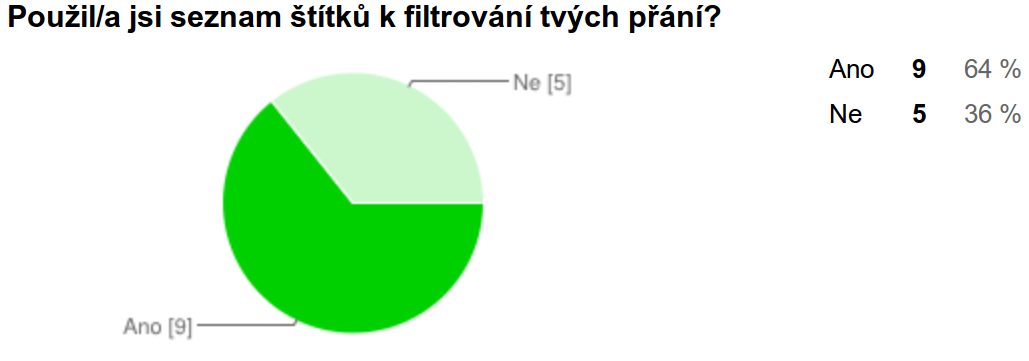
\includegraphics[width=110mm]{./pictures/dotaznik/vice-prani-03.png}
\label{fig:dot:vice-prani-03}
\end{center}
\end{figure}

\section{Práce s přáním}
\begin{figure}[H]
\begin{center}
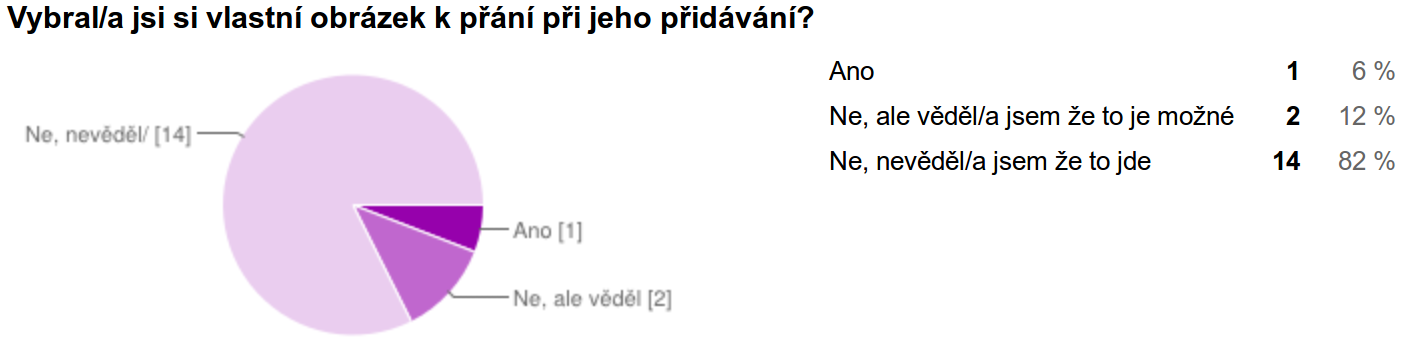
\includegraphics[width=110mm]{./pictures/dotaznik/jedno-prani-01.png}
\label{fig:dot:jedno-prani-01}
\end{center}
\end{figure}

\begin{figure}[H]
\begin{center}
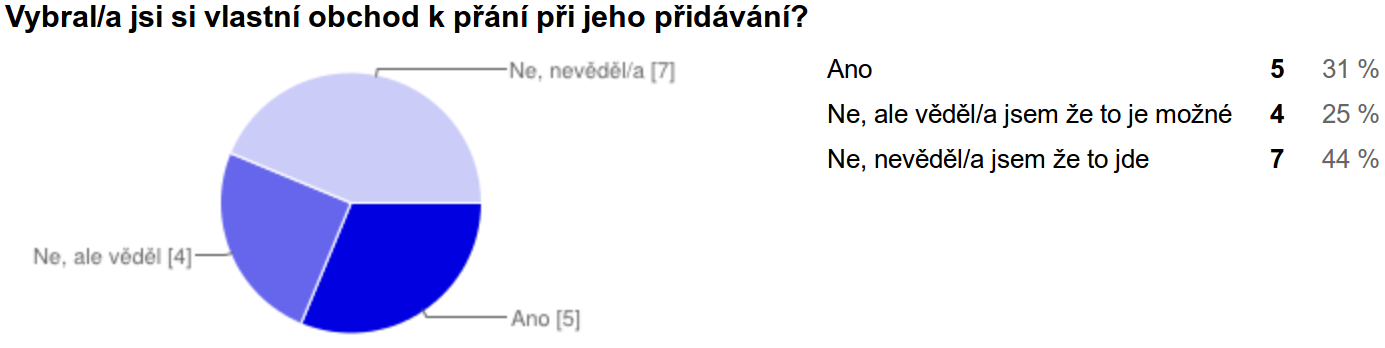
\includegraphics[width=110mm]{./pictures/dotaznik/jedno-prani-02.png}
\label{fig:dot:jedno-prani-02}
\end{center}
\end{figure}

\begin{figure}[H]
\begin{center}
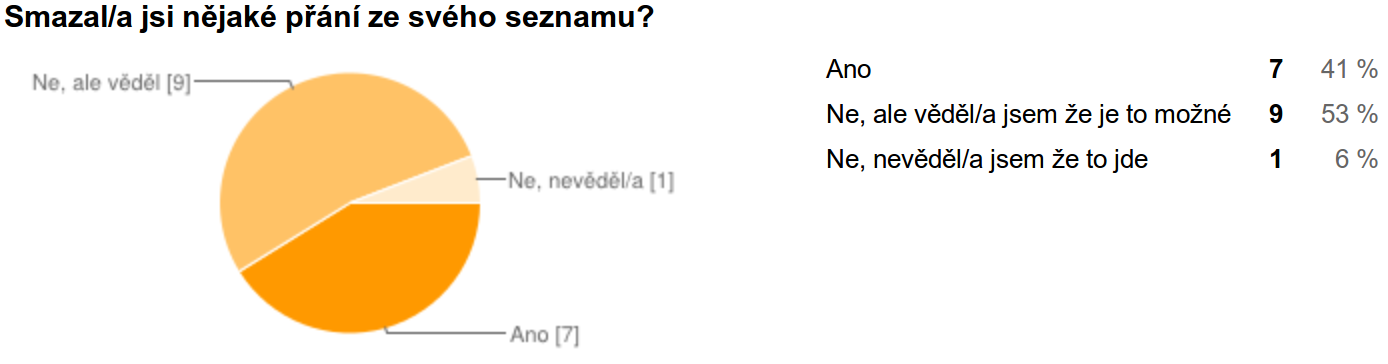
\includegraphics[width=110mm]{./pictures/dotaznik/jedno-prani-03.png}
\label{fig:dot:jedno-prani-03}
\end{center}
\end{figure}

\begin{figure}[H]
\begin{center}
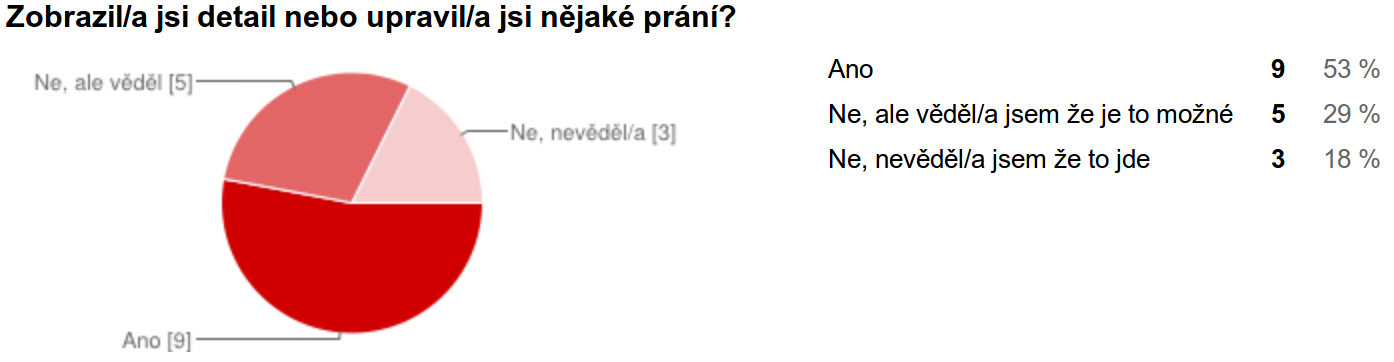
\includegraphics[width=110mm]{./pictures/dotaznik/jedno-prani-04.png}
\label{fig:dot:jedno-prani-04}
\end{center}
\end{figure}

\begin{figure}[H]
\begin{center}
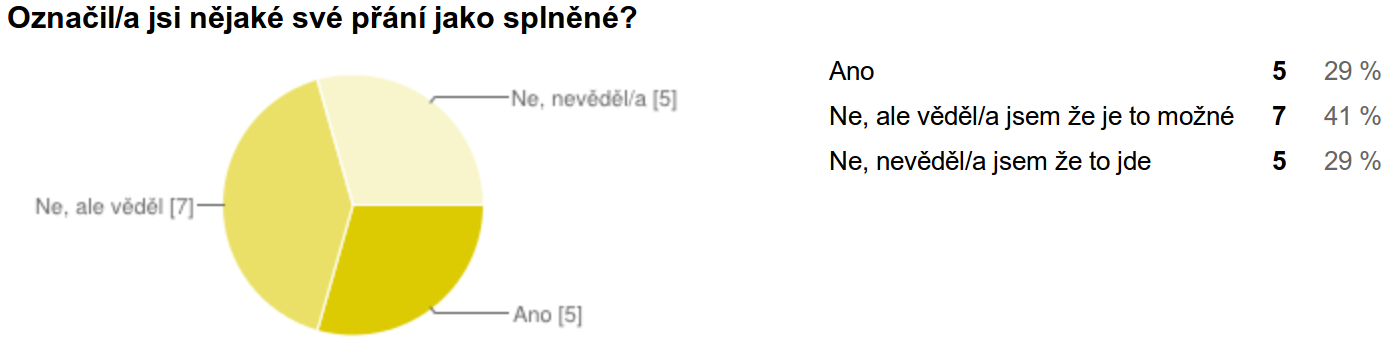
\includegraphics[width=110mm]{./pictures/dotaznik/jedno-prani-05.png}
\label{fig:dot:jedno-prani-05}
\end{center}
\end{figure}

\begin{figure}[H]
\begin{center}
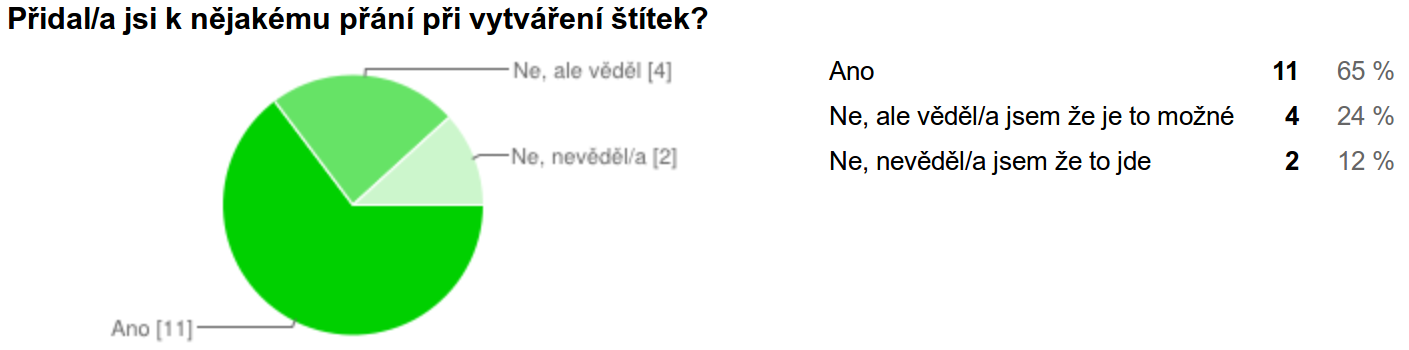
\includegraphics[width=110mm]{./pictures/dotaznik/jedno-prani-06.png}
\label{fig:dot:jedno-prani-06}
\end{center}
\end{figure}